\documentclass{article}
\usepackage{amsmath}
\usepackage{amsfonts}

\usepackage{tikz}
\usetikzlibrary{fit,positioning,shapes}

\usepackage[shortlabels]{enumitem}

\usepackage{algorithm}
\usepackage{amssymb}
\usepackage{booktabs}
\usepackage{algpseudocode}

\textwidth=7.6in
\textheight=9.9in
\topmargin=-.9in
\headheight=0in
\headsep=.5in
\hoffset=-1.5in
\setlength\parindent{0pt}


\begin{document}

\begin{center}
    \Large{\textbf{Problem Set 2 Solutions}} \\[0.25ex]
    Calvin Walker
\end{center}
\textbf{1.}
\begin{enumerate}[(a)]
    \item \begin{align*}
        P(E) &= \sum_{r, m, h, s, b, a, l}P(r, m, h, s, b, a, l, E) \\ 
        &=  \sum_{r, m, h, s, b, a, l} P(r) P(m) P(h | r, m) P(s | h) P(a | h) P(b | h) P(E | s, b) P(l | b, a) \\
        &= \sum_{b}\sum_{s} P(E|s, b) \sum_{h} P(s | h) P(b | h) \sum_{a} P(a | h) \sum_{l} P(l | b, a) \sum_{r} P(r)\sum_{m} P(h | r, m) P(m)
    \end{align*}
    \item The corresponding elimination ordering is $\prec= M, R, L, A, H, S, B$
    \item \textcolor{white}{{x}}
    \begin{figure}[h]
        \centering
        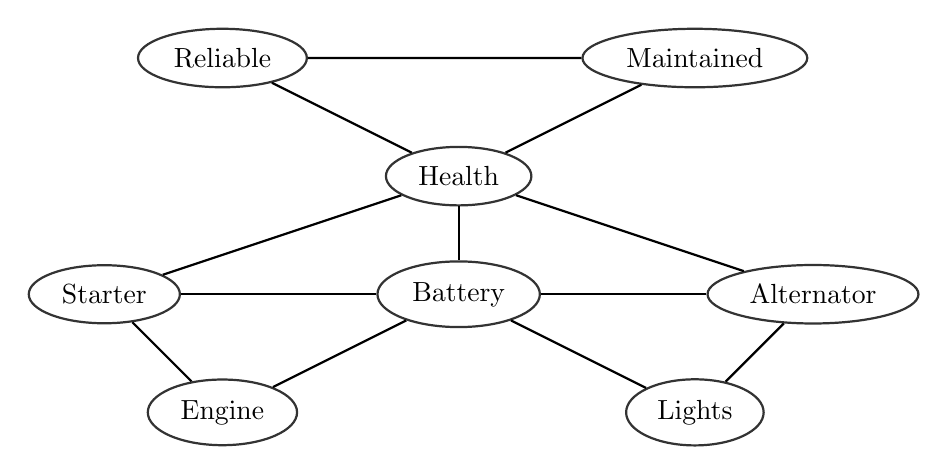
\begin{tikzpicture}[xscale=3.0,yscale=1.5]
            \tikzstyle{latent}=[ellipse, minimum size = 5mm, inner sep=4pt, thick, draw = black!80, node distance = 10mm]
            \tikzstyle{connect}=[thick]
            \node[latent] (R) at (-1,2){Reliable};
            \node[latent] (M) at (1,2){Maintained};
            \node[latent] (H) at (0,1){Health};
            \node[latent] (S) at (-1.5,0){Starter};
            \node[latent] (B) at (0,0){Battery};
            \node[latent] (A) at (1.5,0){Alternator};
            \node[latent] (E) at (-1,-1){Engine};
            \node[latent] (L) at (1,-1){Lights};
            \path[-] (R) edge [connect] (H);
            \path[-] (R) edge [connect] (M);
            \path[-] (S) edge [connect] (B);
            \path[-] (B) edge [connect] (A);
            \path[-] (M) edge [connect] (H);
            \path[-] (H) edge [connect] (S);
            \path[-] (H) edge [connect] (B);
            \path[-] (H) edge [connect] (A);
            \path[-] (S) edge [connect] (E);
            \path[-] (B) edge [connect] (E);
            \path[-] (B) edge [connect] (L);
            \path[-] (A) edge [connect] (L);
        \end{tikzpicture}
        \caption{Moralized graph for the Bayesian Network} \label{fig:auto-bn}
    \end{figure}
    \item The initial set of factors is $\Phi = \{\phi(H, M, R), \phi(S, B, H), \phi(H, B, A), \phi(S, B, E), \phi(B, A, L)\}$ 
    % Step 1: Eliminate $M$ \begin{enumerate}[(i)]
    %     \item $\psi_1(H, M, R) = \phi(H, M, R)$,  
    %     \item Variables involved: $H, M, R$
    %     \item $\tau_1(H, R)  = \sum_{m}\phi_1(H, m, R)$
    % \end{enumerate}
    \begin{table}[h!]
        \centering
        \begin{tabular}{|c|c|c|c|c|}
          \hline
        %   \multirow{2}{*}{Header 1} & \multicolumn{2}{c|}{Header 2} & \multirow{2}{*}{Header 3} & \multirow{2}{*}{Header 4} \\
          Step & Variable & Intermediate & Variables & New  \\
               & Eliminated & Factor & Involved & Factor \\
          \hline
          1 & $M$ & $\psi_1(H, M, R) = \phi(H, M, R)$ & $H, M, R$ & $\tau_1(H, R) = \sum_{m}\psi_1(H, m, R)$ \\
          2 & $R$ & $\psi_2(H, R) = \tau_1(H, R)$ & $H, R$ & $\tau_2(H) = \sum_{r}\psi_2(H, r)$ \\
          3 & $L$ & $\psi_3(B, A, L) = \phi(B, A, L)$ & $B, A, L$ & $\tau_3(B, A) = \sum_{l}\psi_3(B, A, l)$ \\
          4 & $A$ & $\psi_4(A, B, H) = \tau_3(B, A)\phi(H, B, A)$ & $H, B, A$ & $\tau_4(B, H) = \sum_{a}\psi_4(a, B, H)$ \\
          5 & $H$ & $\psi_5(S, B, H) = \tau_2(H)\tau_4(B, H)\phi(S, B, H)$ & $S, B, H$ & $\tau_5(S, B) = \sum_{h}\psi_5(S, B, h)$ \\
          6 & $B$ & $\psi_6(S, B, E) = \tau_5(S, B)\phi(S, B, E)$ & $S, B, E$ & $\tau_6(S, E) = \sum_{l}\psi_6(S, b, E)$ \\
          7 & $S$ & $\psi_6(S, E) = \tau_6(S, E)$ & $S, E$ & $\tau_7(E) = \sum_{s}\psi_7(s, E)$ \\
          \hline
        \end{tabular}
        \caption{Variable Elimination Procedure for $P(E)$}
        \label{tab:example}
      \end{table}
      \item The largest induced scope is $2$, and assuming each variable can take $k$ possible values, the computational complexity would be $O(nk^2)$, since the factor has $k^2$ entries. 
      \item The induced graph is the same as the moralized netowrk in part $(c)$, since there are already edges between all variables appearing in some $\psi$ generated by the variable elimination.
      \newpage
      \item Since the ordering in part $(b)$ produced the most efficient variable elimination in part $(d)$, the associated clique tree is that of part $(d)$, shown below: 
      \begin{figure}[h]
        \centering
        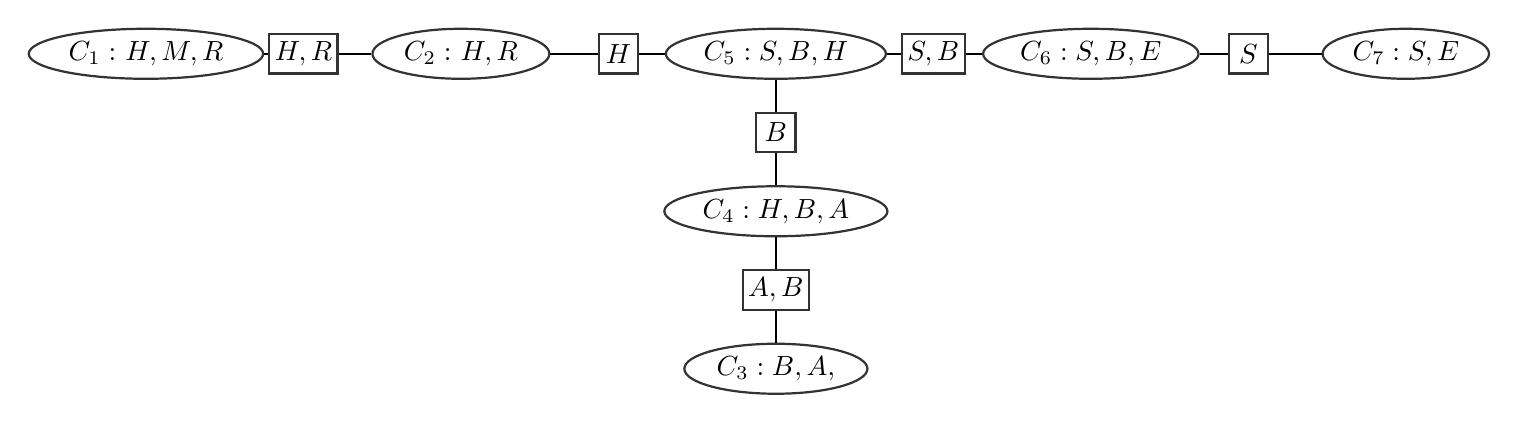
\begin{tikzpicture}[xscale=2.0,yscale=1.0]
            \tikzstyle{clique}=[ellipse, minimum size = 5mm, inner sep=2pt, thick, draw = black!80, node distance = 10mm]
            \tikzstyle{sepset}=[rectangle, minimum size = 5mm, inner sep=2pt, thick, draw = black!80, node distance = 10mm]
            \tikzstyle{connect}=[thick]
            \node[clique] (C1) at (-4,2){$C_1:$ $H, M, R$};
            \node[sepset] (S12) at (-3,2){$H, R$};
            \node[clique] (C2) at (-2,2){$C_2:$ $H, R$};

            \node[sepset] (S25) at (-1,2){$H$};
            \node[clique] (C5) at (0,2){$C_5:S, B, H$};
            \node[sepset] (S45) at (0,1){$B$};
            \node[clique] (C4) at (0,0){$C_4:H, B, A$};
            \node[sepset] (S34) at (0,-1){$A, B$};
            \node[clique] (C3) at (0,-2){$C_3:B, A, $};
            
            \node[sepset] (S56) at (1,2){$S, B$};
            \node[clique] (C6) at (2,2){$C_6:S, B, E$};
            \node[sepset] (S67) at (3,2){$S$};
            \node[clique] (C7) at (4,2){$C_7:S, E$};
            \path[-] (C1) edge [connect] (S12);
            \path[-] (S12) edge [connect] (C2);
            \path[-] (C2) edge [connect] (S25);
            \path[-] (S25) edge [connect] (C5);
            \path[-] (C3) edge [connect] (S34);
            \path[-] (S34) edge [connect] (C4);
            \path[-] (C4) edge [connect] (S45);
            \path[-] (S45) edge [connect] (C5);
            \path[-] (S25) edge [connect] (C5);
            \path[-] (C5) edge [connect] (S56);
            \path[-] (S56) edge [connect] (C6);
            \path[-] (C6) edge [connect] (S67);
            \path[-] (S67) edge [connect] (C7);

        \end{tikzpicture}
        \caption{Clique Tree for the Bayesian Network}
    \end{figure}
      \item If we first eliminate $H$, there is an induced scope of $5$, as we create a new factor $\tau_1(R, M, S, B, A)$, next we could eliminate $B$, to induce a scope of $6$, as we create a new factor $\tau_2(R, M, S, A, E, L)$ with the remaining $6$ random variables. So any elimination ordering starting $\prec = H, B \dots$ would lead to a computational complexity of $O(nk^6)$
\end{enumerate}
\textbf{2.}
\begin{enumerate}[(a)]
    \item Consider two clusters $C_i$ and $C_k$ in $\cal{T}$, a cluster tree for the graph $\cal{H}$, and a variable $X$ that is eliminated at $C_k$. If $W_{<(i, j)}$ and $W_{<(j, i)}$ are seperated given $S_{i,j}$ in $\cal{H}$, then no clusters upstream from $C_k$ can contain $X$, since $X$ is not in the sepset of any upsteam cluster of $C_k$. We know $X$ must be present in the message $m_{i \rightarrow j}$ to the next cluster from $C_i$, and this message is multiplied into the ensuing messages (so these clusters have $X$ in their scope) until we reach $C_k$. Thus, $X$ is in the scope of the unique path from $C_i$ to $C_k$, and $\cal{T}$ satisfies the running intersection property. \\[0.75ex]
    Assume that the cluster tree $\cal{T}$ satisfies the running intersection property, so for some clusters $C_i$ and $C_k$ with a variable $X$ that is eliminated at $C_k$, $X$ must be in every cluster in the unique path from $C_i$ to $C_k$. Thus, it is also in the sepset between each clique along this unique path. If $X$ is not in the sepset between two cliques $C_i$ and $C_j$, then $X$ cannot be upstream of $C_j$, so $W_{<(i, j)}$ and $W_{<(j, i)}$ must be seperated given $S_{i,j}$ if $\cal{T}$ satisfies the running intersection property. 
    \item Variable elimination produces an induced chordal graph $\mathcal{I}_{\Phi, \prec}$ that contains $\mathcal{H}$. We know by the definition of $\mathcal{I}_{\Phi, \prec}$ that the scope of every generated factor $\psi$, which are the nodes of $\cal{T}$, is a clique in $\mathcal{I}_{\Phi, \prec}$. Now, let $\mathbf{X} = \{X_1 \dots X_n\}$ be a maximal clique in $\mathcal{I}_{\Phi, \prec}$, and $X_1$ the first variable from $\bf{X}$ in $\prec$. Then there are edges between $X_1$ and all $X_i \in \bf{X}$ before eliminating $X_1$, so there exist factors $\phi_{X_1}(X_1, X_i)$ for all $X_i \in \bf{X}$. To eliminate $X_1$, we must create a factor $\psi$ that contains $X_1 \dots X_n$ and no other variables outside the clique (or otherwise they would be in $\mathbf{X}$), So every maximal clique in $\mathcal{I}_{\Phi, \prec}$ is the scope of some factor $\psi$, and thus a node in $\cal{T}$.
    \item 
    Consider the joint distribution between the variables in three cliques $\mathbf{Y} = \{C_i, C_j, C_k\}$ such that $C_i$ neighbors $C_j$ and $C_j$ neighbors $C_k$: \begin{align*}
        P(\mathbf{Y}) &= P(C_i \setminus \{S_{ij}\}, C_j \setminus \{S_{ij}, S_{jk}\}, C_k \setminus \{S_{jk}\}, S_{ij}, S_{jk})
    \end{align*}
    Where the vairables not in the sepsets are conditionally independent in two neighboring cliques, so 
    \begin{align*}
        P(\mathbf{Y}) &= P(C_i \setminus \{S_{ij}\} | S_{ij}) P(C_j \setminus \{S_{ij}, S_{jk}\}| S_{jk},S_{ij})P(S_{ij}) P(C_k \setminus \{S_{jk}\} | S_{jk})P(S_{jk}) \\[0.5ex]
        &= \frac{P(C_i)}{P(S_{ij})}\frac{P(C_j)}{P(S_{ij})P(S_{jk})}\frac{P(C_k)}{P(S_jk)}P(S_{ij})P(S_{jk}) \\[1.0ex]
        &= \frac{P(C_i) P(C_j)P(C_k)}{P(S_{ij})P(S_{jk})}
    \end{align*}
    So we can extend this process over the clique tree to compute the joint distribution as: \begin{align*}
        P(\mathbf{X}) = \frac{\prod_{i}P(C_i)}{\prod_{ij}P(S_{ij})}
    \end{align*}
    \item Either $\cal{T}' = \cal{T}$ or there are $C_i, C_j \in \cal{T}$ such that $C_i \subseteq C_j$. If we eliminate $C_i$, $\cal{T}'$ is family preserving since Scope$[\phi_i] \subseteq C_i \subseteq C_j$. We connect all neighbors of $C_i$ to $C_j$ when removing $C_i$, so any path through $C_i$ is preserved via $C_j$ since there can be no $X \in C_i$ not in $C_j$. Thus, if $\cal{T}$ satisfies the running intersection property, so does $\cal{T}'$
\end{enumerate}
\textbf{3.} 
\begin{enumerate}[(a)]
    \item We can follow the algorithim for out of clique inference in a clique tree to solve for $P(X_i, X_j)$, given a calibrated clique tree $\cal{T}$. First we define $\cal{T}'$ to be the subtree of $\cal{T}$ such that $(X_i, X_j) \subseteq Scope[\cal{T}']$, then define a new set of factors (letting $C_j$ be the root): \begin{equation*} 
        \Phi = \{\beta_j\} \cup \{ \phi_k = \frac{\beta_k}{\mu_{k, k + 1}} \ | \ k \in \mathcal{V}_{\cal{T'}} - \{j\} \}
    \end{equation*}
    Which can be done in linear time. Then we perform sum-product variable elimination on a ordering $\prec= X_{i + 1} \dots X_{j - 1}$ of $\mathbf{Z} = Scope[\mathcal{T'}] - \{X_i, X_j\}$. The running time of the variable elimination is $O(nk)$ since the largest induced width is one. 
    \item Naively, we must run the $O(nk)$ process for all $\binom{n}{2}$ combinations of $i$ and $j$, so the running time would be $O(n^3k)$
    \item Following the procedure in part $(a)$, perform variable elimination on the ordering $\prec =X_2, X_3 $ and set of factors $\Phi = \{\beta_3(X_3, X_4), \frac{\beta_1(X_1, X_2)}{\mu_{1, 2}(X_2)}, \frac{\beta_2(X_2, X_3)}{\mu_{2, 3}(X_3)}\}$. So \begin{align*}
        P(X_1, X_4) &= \sum_{X_3} \frac{\beta_3(X_3, X_4)}{\mu_{2, 3}(X_3)} \sum_{X_2}\frac{\beta_1(X_1, X_2)\beta_2(X_2, X_3)}{\mu_{1, 2}(X_2)} \\[1.0ex]
        &= \sum_{X_3} \frac{\beta_3(X_3, X_4)}{\mu_{2, 3}(X_3)} P(X_1, X_3)
    \end{align*}
    Thus, if we cache $P(X_1, X_3)$, we can compute $P(X_1, X_4)$ more efficiently since we avoid re-computing $P(X_1, X_3)$
    \item From part $(c)$, we can observe the simple recurrence relation: \begin{equation*}
        P(X_i, X_j) = \sum_{X_j - 1} \frac{\beta_{{j - 1}}(X_{j - 1}, X_j)}{\mu_{{j - 2}, {j - 1}}(X_{j - 1})}P(X_i, X_{j - 1})
    \end{equation*}
    A dynamic programming algorithm would be, for each $i \in [n - 2]$, cache the result of $P(X_i, X_{i + 2})$, and then use this to iterativley compute $P(X_i, X_{i + 3}), P(X_i, X_{i + 3}), \dots ,P(X_i, X_{n})$ using the above recurrence relation (and caching the last computed result). This process would take $O(nk)$ time for each $i$, so the total running time of the algorithim is $O(n^2k)$.
\end{enumerate}
\textbf{4.} \begin{enumerate}[(a)]
    \item \begin{align*}
        \mathcal{N}^{-1}(x; \eta_1, \lambda_1) \cdot \mathcal{N}^{-1}(x; \eta_1, \lambda_1) &= \sqrt{\frac{\lambda_1}{2\pi}}\exp(-\frac{1}{2}(\lambda_1x^2 - 2x\eta_1 + \lambda_1\mu^2)) \cdot \sqrt{\frac{\lambda_2}{2\pi}}\exp(-\frac{1}{2}(\lambda_2x^2 - 2x\eta_2 + \lambda_2\mu^2)) \\
        &\propto \exp(-\frac{1}{2}((\lambda_1x^2 - 2x\eta_1) + (\lambda_2x^2 - 2x\eta_2))) \\
        &= \exp(-\frac{1}{2}((\lambda_1 + \lambda_2)x^2 + 2x(\eta_1 - \eta_2))) \\
        % &= \exp(-\frac{1}{2}(x^2 + 2x\frac{\eta_1 + \eta_2}{\lambda_1 + \lambda_2} + \frac{\lambda_1\eta_1 + \lambda_2\eta_2}{\lambda_1 + \lambda_2})) \\
        &= \exp(-\frac{1}{2}(\bar{\lambda}x^2 + 2x\bar{\eta})) \propto \mathcal{N}^{-1}(x;\bar{\eta}, \bar{\lambda})
    \end{align*}
    \item \begin{align*}
        m_{j \rightarrow i} &= \sum_{x_j} \psi_j(x_i, x_j) \prod_{k \in \text{Nb}(j) \setminus \{i\}}m_{k \rightarrow j} \\
        &= \sum_{x_j} \phi(x_j) \phi(x_i, x_j) \prod_{k \in \text{Nb}(j) \setminus \{i\}} \sum_{x_k} \exp(-\frac{1}{2}(\Lambda_{kk}x_k^2 + 2\eta_kx_k)  - \Lambda_{kj}x_kx_j) \prod_{l \in \text{Nb}(k)\setminus \{j\}} m_{l \rightarrow k}(x_k) \\
        &= \sum_{x_j} \exp(-\frac{1}{2}(\Lambda_{jj}x_j^2 + 2\eta_jx_j)  - \Lambda_{ji}x_jx_i) \prod_{k \in \text{Nb}(j) \setminus \{i\}} \sum_{x_k} \mathcal{N}^{-1}([x_k, x_j]; \eta_k, \Lambda_k)\ \mathcal{N}^{-1}(x_k; \bar{\eta}, \bar{\Lambda})\\
        &= \sum_{x_j} \mathcal{N}^{-1}([x_j, x_i]; \eta_j, \Lambda_j)\ \mathcal{N}^{-1}(x_j ; \bar{\eta}_k, \bar{\Lambda}_k) \\
        &= \mathcal{N}^{-1}(x_i; \bar{\eta}_j, \bar{\Lambda}_j)
    \end{align*}
    \item The belief at node $i$ is the product of the incoming messages:
    \begin{align*}
        \beta(x_i) = \prod_{j \in \text{Nb}_{i}} m_{j \rightarrow i}
    \end{align*}
    Which we can see from part (b) is a product of Gaussians with node $i$'s neighbors marginalized out. So, 
    \begin{align*}
        \beta(x_i) = \mathcal{N}^{-1}(x_i; \bar{\eta}, \bar{\Lambda})
    \end{align*}
\end{enumerate}

\textbf{5.1}\begin{enumerate}[(a)]
    \item \begin{figure}[h]
        \centering
        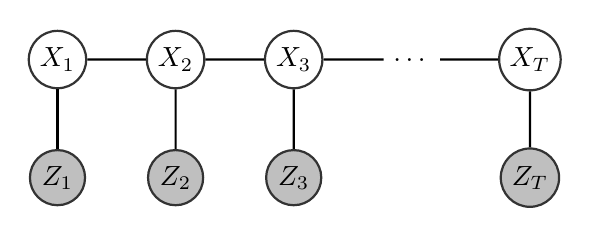
\begin{tikzpicture}[xscale=1.5,yscale=1.5]
                \tikzstyle{latent}=[circle, minimum size = 7mm, inner sep=2pt, thick, draw = black!80, node distance = 10mm]
                \tikzstyle{observed}=[circle, minimum size = 7mm, inner sep=2pt, thick, draw = black!80, node distance = 10mm,fill=gray!50]
                \tikzstyle{connect}=[thick]
                \node[latent] (x1) at (0,1){$X_1$};
                \node[latent] (x2) at (1,1){$X_2$};
                \node[latent] (x3) at (2,1){$X_3$};
                \node (xdot) at (3,1){\ldots};
                \node[latent] (xt) at (4,1){$X_T$};
    \node[observed] (z1) at (0,0){$Z_1$};
                \node[observed] (z2) at (1,0){$Z_2$};
                \node[observed] (z3) at (2,0){$Z_3$};
    \node[observed] (zt) at (4,0){$Z_T$};
                \path[-] (x1) edge [connect] (x2);
                \path[-] (x2) edge [connect] (x3);
                \path[-] (x3) edge [connect] (xdot);
                \path[-] (xdot) edge [connect] (xt);
                \path[-] (x1) edge [connect] (z1);
                \path[-] (x2) edge [connect] (z2);
                \path[-] (x3) edge [connect] (z3);
                \path[-] (xt) edge [connect] (zt);
    
    \end{tikzpicture}
            \caption{Undirected Hidden Markov model}\label{fig:hmm}
    \end{figure}
    $\Phi = \{\phi(X_1) = P(X_1),\ \phi(X_t, Z_t) = P(Z_t | X_t),\ \phi(X_{t - 1}, X_t) = P(X_t | X_{t - 1})\}$
    \item \textcolor{white}{{x}}\begin{figure}[h]
        \centering
        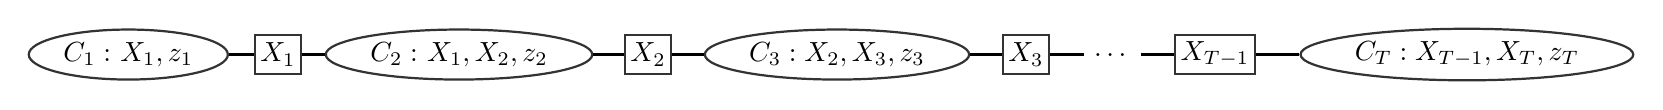
\begin{tikzpicture}[xscale=2.0,yscale=1.0]
            \tikzstyle{clique}=[ellipse, minimum size = 5mm, inner sep=2pt, thick, draw = black!80, node distance = 10mm]
            \tikzstyle{sepset}=[rectangle, minimum size = 5mm, inner sep=2pt, thick, draw = black!80, node distance = 10mm]
            \tikzstyle{connect}=[thick]
            \node[clique] (C1) at (-4,2){$C_1:$ $X_1, z_1$};
            \node[sepset] (S12) at (-3.05,2){$X_1$};
            \node[clique] (C2) at (-1.9,2){$C_2:$ $X_1, X_2, z_2$};
            \node[sepset] (S23) at (-0.7,2){$X_2$};
            \node[clique] (C3) at (0.5,2){$C_3: X_2, X_3, z_3$};
            \node[sepset] (S3d) at (1.7,2){$X_3$};
            \node (xdot) at (2.25,2){\ldots};
            \node[sepset] (SdT) at (2.9,2){$X_{T - 1}$};
            % \node[sepset] (S45) at (0,1){$B$};
            % \node[clique] (C4) at (0,0){$C_4:H, B, A$};
            % \node[sepset] (S34) at (0,-1){$A, B$};
            % \node[clique] (C3) at (0,-2){$C_3:B, A, $};
            
            % \node[sepset] (S56) at (1,2){$S, B$};
            % \node[clique] (C6) at (2,2){$C_6:S, B, E$};
            % \node[sepset] (S67) at (3,2){$S$};
            \node[clique] (CT) at (4.5,2){$C_T: X_{T - 1}, X_T, z_T$};
            \path[-] (C1) edge [connect] (S12);
            \path[-] (S12) edge [connect] (C2);
            \path[-] (C2) edge [connect] (S23);
            \path[-] (S23) edge [connect] (C3);

            \path[-] (C3) edge [connect] (S3d);
            \path[-] (S3d) edge [connect] (xdot);
            \path[-] (xdot) edge [connect] (SdT);
            \path[-] (SdT) edge [connect] (CT);

            % \path[-] (C3) edge [connect] (xdot);
            % \path[-] (C3) edge [connect] (S34);
            % \path[-] (S34) edge [connect] (C4);
            % \path[-] (C4) edge [connect] (S45);
            % \path[-] (S45) edge [connect] (C5);
            % \path[-] (S25) edge [connect] (C5);
            % \path[-] (C5) edge [connect] (S56);
            % \path[-] (S56) edge [connect] (C6);
            % \path[-] (C6) edge [connect] (S67);
            % \path[-] (S67) edge [connect] (C7);

        \end{tikzpicture}
        \caption{Clique Tree for the Undirected HMM}
    \end{figure}
    \item We can easily compute the first two messages: \begin{align*}
        m_{1 \rightarrow 2}(X_1) &= \phi(X_1, z_1) = P(X_1, z_1), \\
        m_{2 \rightarrow 3}(X_2) &= \sum_{X_1}\phi(X_1, X_2) \phi(X_2, z_2) m_{1 \rightarrow 2}(X_1) = \sum_{X_1}P(X_2 | X_1)P(z_2 | X_2) P(X_1, z_1)
    \end{align*}
    So a general expression for $t \rightarrow t + 1$ is:
    \begin{align*}
        m_{t \rightarrow t + 1}(X_t) &= \sum_{X_{t - 1}} \phi(X_{t -1}, X_{t})\phi(X_{t}, z_{t}) m_{t - 1 \rightarrow t}(X_{t - 1}) \\
        &= \sum_{X_{t - 1}} P(X_{t} | X_{t - 1})P(z_t | X_t) m_{t - 1 \rightarrow t}(X_{t - 1})
    \end{align*}
    Where $m_{t - 1 \rightarrow t}(X_{t - 1}) = P(X_{t - 1}, z_1, z_2, \dots ,z_{t - 1})$. Thus, $m_{t\rightarrow t + 1}(X_t) = P(X_{t}, z_1, z_2, \dots ,z_{t})$
    \item Starting with the first message: \begin{align*}
        m_{T \rightarrow T - 1}(X_{T - 1}) &= \sum_{X_T}\phi(X_{T - 1}, X_T)\phi(X_T, z_T) \\
        &= \sum_{X_T} P(X_T | X_{T - 1})P(z_T | X_T)
    \end{align*}
    So a general expression for $t + 1 \rightarrow t$ is: \begin{align*}
        m_{t + 1 \rightarrow t}(X_t) &= \sum_{X_{t + 1}}\phi(X_t, X_{t + 1})\phi(X_{t + 1}, z_{t})m_{t + 2 \rightarrow t + 1}(X_{t + 1}) \\
        &= \sum_{X_{t + 1}}P(X_{t + 1} | X_t)P(z_{t + 1}|X_{t + 1})m_{t + 2 \rightarrow t + 1}(X_{t + 1})\\
        &= \sum_{X_{t + 1}}P(X_{t + 1} | X_t)P(z_{t + 1}|X_{t + 1})P(z_{t + 2}, z_{t + 3}, \dots , z_T | X_{t + 1})\\
        &= P(z_{t + 1}, z_{t + 2}, \dots , z_T | X_{t})
    \end{align*}
    \item \begin{align*}
        P(X_t | z_1, z_2, \dots , z_T) &= \frac{P(X_t, z_1, z_2, \dots , z_T)}{P(z_1, z_2, \dots , z_T)} \\[0.75ex]
        &= \frac{P(z_{t + 1}, z_{t + 2}, \dots , z_T | X_t)P(X_t, z_1, z_2, \dots , z_t)}{\sum_{X}P(\mathbf{X}, \mathbf{z})} \\[0.75ex]
        &= \frac{m_{t + 1 \rightarrow t}(X_t)m_{t \rightarrow t + 1}(X_t)}{\sum_X\phi(X_1, z_1)\prod_{t = 2}^T\phi(X_{t - 1}, X_t)\phi(X_t, z_t)}
    \end{align*}
\end{enumerate}
\textbf{5.2}\begin{enumerate}[(a)]
    \item 
    \begin{align*}
        \alpha_t(X_t) &= P(Z_1, \dots, Z_t, X_t) = \sum_{X_{t - 1}}P(Z_1, \dots, Z_t, X_{t - 1}, X_t) \\
        &= \sum_{X_{t - 1}}P(Z_t |Z_1, \dots, Z_{t - 1}, X_t, X_{t - 1}) P(X_t | Z_1, \dots, Z_{t - 1}, X_{t - 1}) P(Z_1, \dots, Z_{t - 1}, X_{t - 1}) \\
        &= \sum_{X_{t - 1}}P(Z_t | X_t) P(X_t | X_{t - 1}) \alpha_{t - 1}(X_{t - 1})
    \end{align*}
    Where $\alpha_1(X_1) = P(Z_1 | X_1) P(X_1)$
    \item \begin{align*}
        \beta_t(X_t) &= P(Z_{t + 1}, \dots, Z_T | X_t)\sum_{X_{t + 1}}P(Z_{t + 1}, \dots, Z_T, X_{t + 1} | X_t) \\ 
        &= \sum_{X_{t + 1}}P(Z_{t + 2} \dots Z_T | X_{t + 1}, X_t, Z_{t + 1}) P(Z_{t + 1} | X_{t + 1}, X_{t})P(X_{t + 1} | X_{t}) \\
        &= \sum_{X_{t + 1}}P(Z_{t + 2} \dots Z_T | X_{t + 1}) P(Z_{t + 1} | X_{t + 1})P(X_{t + 1} | X_{t}) \\ 
        &= \sum_{X_{t + 1}}\beta_{t + 1}(X_{t + 1}) P(Z_{t + 1} | X_{t + 1})P(X_{t + 1} | X_{t})
    \end{align*}
    \item Similar 5.1 (e) we have that  $P(X_t | Z_1, \dots , Z_T) \propto P(X_t, Z_1,\dots,Z_T) = P(Z_{t + 1}, \dots , Z_T | X_t)P(X_t, Z_1, \dots,Z_t) = \beta_t(X_t)\alpha_t(X_t)$
    \item $\beta_t(X_t) = P(Z_{t + 1}, \dots , Z_T | X_t) = m_{t + 1 \rightarrow t}(X_t)$ and $\alpha_t(X_t) = P(X_t, Z_1, \dots,Z_t) = m_{t \rightarrow t + 1}(X_t)$
\end{enumerate}
\textbf{6}\begin{enumerate}[(a)]
    \item I did not collaborate 
    \item 10 - 20 hours
\end{enumerate}
\end{document}